\chapter{Calibrations}

\indent This chapter addresses the calibrations of all the detectors. The process involved converting raw signals from the detectors into real physical quantities allowing for the energy, position and timing corrections to be determined and applied in the subsequent analysis.

\section{Tagger Energy Calibrations}

\indent The tagger energy calibration determines the relation between tagger channel number and electron energy. The calibrations were carried out by the colleagues at the University of Glasgow \cite{mcgeorge}.

\indent In order to make a tagger energy calibration, an incident MAMI electron beam of an energy of interest is bent in the magnetic field; for a 855MeV beam, field of ~1.025T is used. Then the magnetic field was varied in small steps to guide the beam through the focal plane and an energy measurement was taken at each step. Six different electron beam energies were used for the calibration, they ranged from 195.22MeV to 705.26 MeV, with the uncertainty of 0.16MeV; the uncertainty in the magnetic field was 0.01mT \cite{duncan}.

\indent The varying magnetic field required to sweep the beam across a given channel allowed for the determination of a position of a  hit in a FP detector with an accuracy of 0.05 channel width. Finally, in order to relate the the FP channel number to the electron energy a linear interpolation between different energies was used.

\section{Crystal Ball Calibrations}

\subsection{Clustering Algorithm}

\indent Photons entering Crystal Ball deposit their energy in the NaI crystals via electromagnetic showers which hit multiple crystals in each event.These groups of hit crystals are called clusters. The accurate analysis of the CB events required an algorithm which identifies the clusters and recovers information about the incident photon's energy and position from the energy deposited in the crystals within a cluster.

\indent First step in the analysis is to identify a crystal with the highest energy deposit, central crystal of the cluster, and it's 12 closest neighbors (Fig. \ref{cbcluster}). A hit in this central crystal provides the timing information for the event. The energies of the neighboring crystals are scanned and if their energies are greater than the threshold energy of around 2MeV they are added to the cluster. Only 12 closest neighbors of the central crystal are considered in the algorithm because it has been confirmed that in 98\% of the cases the energy deposit of the shower triggers only 13 crystals \cite{claire}. Then the total energy of the cluster is obtained as:

\begin{equation}
E_{sum}=\Sigma_{k}E_{i}
\end{equation}

where, $E_{i}$ is the energy of the i-th crystal in the cluster of k detector elements. Then the condition of the the total energy of the cluster being greater than 20MeV  is applied to suppress the effects of the background.

\indent The position of the hit is calculated as the weighted mean position given by the below equation:

\begin{equation}
r_{mean}=\frac{\Sigma_{k}\sqrt{E_{i}r_{i}}}{\Sigma_{k}\sqrt{E_{i}}}
\end{equation}

where, $E_{i}$ is the energy deposited in the i-th crystal and $r_{i}$ is the position of the i-th crystal in the cluster.

\begin{figure}[H]
\begin{center}
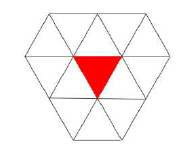
\includegraphics[scale=0.55]{pictures/png/cbcluster.png}
\caption{Schematic representation of a NaI cluster. The central triangle, shaded in red, depicts a triangular face of the NaI crystal and is the logical center of the cluster. The other 12 triangles are its closest neighbors.}
\label{cbcluster}
\end{center}
\end{figure}

\subsection{Energy Calibration}

\indent Crystal Ball energy calibrations have been carried out by the colleagues from UCLA and Johanes Gutenberg Universitaet in Mainz \cite{marc}. The energy calibration of the Crystal Ball was performed in three steps; a low energy calibration - mainly important for the acquisition system was obtained, then a high energy calibration has been performed, and in the end, an energy scale factor has been applied to account for crystal thresholds and clustering algorithms.

\subsubsection{Low energy calibration}

\indent In this first step of the CB energy calibration, an $^{241}$Am/$^{9}$Be source was placed in the center of the Crystal Ball \cite{marc}. The $\alpha$ decay of americium, and a subsequent capture of these particles by beryllium, triggers a series of reactions resulting in the excited state of $^{12}$C which decays to a ground state and emits a 4.438MeV photon in the process. This photon energy deposit in the NaI crystals has been used to adjust the gains of all PMTs, so that the detected peak was in the same position in the ADC spectra for all the detector elements.

\subsubsection{High energy calibration}

\indent The photons produced in meson decay have energies much higher than photons used in the low energy calibration, therefore the calibration for higher energy photons is also required. The $\pi^{0}->\gamma\gamma$ reaction have been used as a source of such photons. The invariant mass, M$_{\gamma\gamma}$, of two photons detected in the CB was reconstructed from the information on the photons measured energy and momentum and only the events with M$_{\gamma\gamma}$ within the mass of $\pi^{0}$ were selected, and the following selection cuts have been applied:

\begin{itemize}
\item no less than 70\% of the detected photon energy had to be deposited in a single NaI crystal. This criterium was decided upon to ensure the deposit in a single crystal dominated the cluster.
\item in order to ensure that the photons used for the calibration were of similar energy, the condition of having the energy difference between two photon clusters being less than 35\% of the total energy have been set up.
\item the tagged photon energy had to be less than 180MeV. This restriction constrained the energy range of the decay photons between 40MeV and 125MeV. Such energy cut favored large opening angles between the photons, resulting in an even angular distributions in the lab.
\end{itemize}

\indent The invariant mass of $\pi^{0}$ has been reconstructed from the two photon decay, and a Gaussian function has been fitted. The mean of the fit, corresponding to M$_{\gamma\gamma}$ , has been compared to the mass of $\pi^{0}$. With this information a new gain factor, $G_{new}$, was obtained according to the below equation:

\begin{equation}
G_{new}=\frac{M_{\gamma\gamma}}{M_{\pi^{0}}}G_{old} [\frac{MeV}{channel}]
\end{equation}

where, $G_{old}$ is the gain factor used previously. Because the detected energy of the photon cluster depended both, on the central crystal and all the other crystals in the cluster a single set of calculation to obtain the new gain was not enough. Several iterations were required for M$_{\gamma\gamma}$ to correspond to M$_{\pi^{0}}$.

\subsubsection{Energy scaling factor}

\indent Because of the energy losses due to individual energy thresholds and the showers, the energy of the incident photons is not the same as the total energy of the cluster. To account for this in the analysis, another energy correction had to be applied. In order to ensure that the mass reconstructed from the decay of two photons was indeed the mass of $\pi^{0}$ meson, a scaling factor of 1.05 was applied to the data.

\subsubsection{Time walk correction}

\indent Because of the slow time response of the NaI crystals, 250ns \cite{knoll}, there arises a time difference between the small and large signals registering at the discriminator threshold. Therefore, the times reported by the TDCs required a correction to account for this time difference and therefore improve the CB time resolution (Fig. \ref{cbtimewalk}). The corrected time, $T_{corr}$, is defined as:

\begin{equation}
T_{corr}=T - r\sqrt{\frac{a_{0}}{a}}
\end{equation}

where, T is the measured time, $a_{0}$ is the discriminator's voltage, r is the rise time and a is the signal's amplitude.

\begin{figure}[H]
\begin{center}
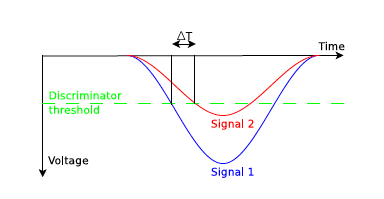
\includegraphics[scale=0.55]{pictures/png/cbtimewalk.png}
\caption{CB time walk.}
\label{cbtimewalk}
\end{center}
\end{figure}

\section{PID Calibration}

\subsection{PID azimuthal correction}

\indent In order to accurately determine the correlation between hits in the PID and Crystal Ball, the PID azimuthal angle ($\phi$) with respect to the Crystal Ball had to be measured. The steps taken to calculate the value of phi are as follows.
\indent First, only the events that triggered signal in one crystal in a CB cluster were selected. The reason for that was to limit the number of photons producing events in more than one crystal and therefore, ensure that only events with clearly determined angles were considered for the calibration. Another cut was made on those events to select only those with just a single reaction in the PID. This way the background due to multi-body final state interactions was highly reduced.
\indent The angular distribution of those events has been plotted for each PID element, which gave a single peak over the azimuthal range of each one (Fig. \ref{pidphi}). A 1D projection has been plotted for each PID element and a Gaussian function was fitted to the peak. Having 24 PID elements means that each of them occupies 15$\deg$ of the total azimuthal coverage. Therefore, a linear fit with a fixed gradient could have been used to accurately determine the PID azimuthal correction (Fig. \ref{pidphi2}).

\begin{figure}[H]
\begin{center}
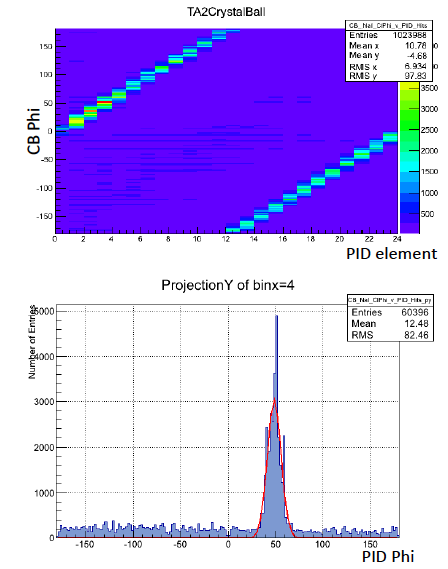
\includegraphics[scale=0.55]{pictures/png/pidphi.png}
\caption{Plot of Phi position in CB cluster vs hit in PID (top) and Gaussian fit to the projection of PID element 4 over the azimuthal range (bottom).}
\label{pidphi}
\end{center}
\end{figure}

\begin{figure}[H]
\begin{center}
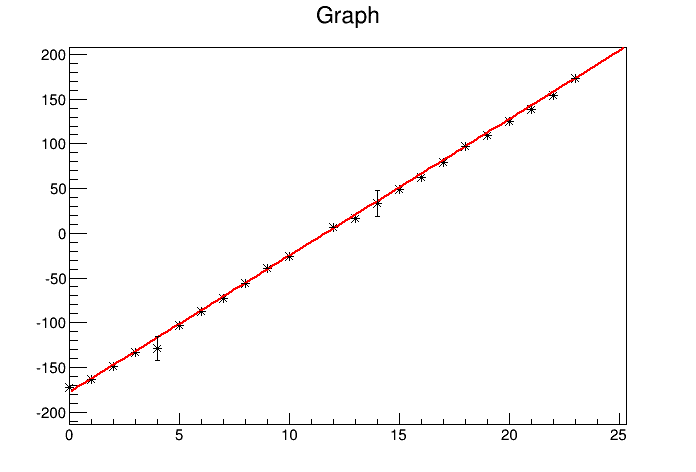
\includegraphics[scale=0.4]{pictures/png/pidcali4.png}
\caption{PID azimuthal correction - linear fit.}
\label{pidphi2}
\end{center}
\end{figure}

\subsection{PID energy correction}

\indent The energy calibration employed banana ($\Delta$E-E) plots described earlier and raw signal from PID ADCs. The banana plots were divided into 10MeV energy bins and projected onto the y-axis (Fig. \ref{bananacali}). Those projections featured two peaks, first one corresponding to the pion and second one representing proton ridges. The latter was fitted with a Gaussian function and the value of the mean has been extracted (Fig. \ref{bananagaus}). This step has been performed for all the energy bins in the range of 20-300MeV. Similarly, the G4 simulated data had the same procedure applied. Subsequently, the means of the Gaussian functions for the experimental data have been plotted against corresponding means for the simulated data and a linear fit has been used to determine the gain for the calibration (Fig. \ref{bananagaus}).

\begin{figure}[H]
\begin{center}
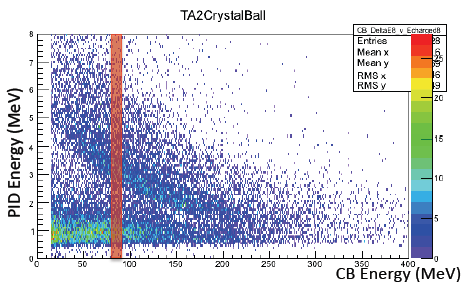
\includegraphics[scale=0.6]{pictures/png/bananacali.png}
\caption{$\Delta$E-E plots of PID vs CB energy deposits. Example10MeV energy bin shaded in red.}
\label{bananacali}
\end{center}
\end{figure}

\begin{figure}[H]
\begin{center}
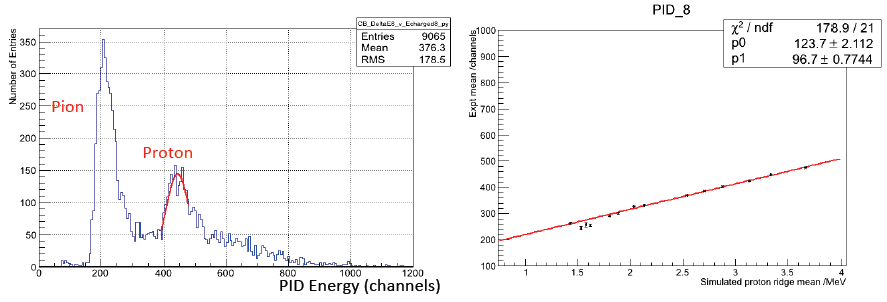
\includegraphics[scale=0.5]{pictures/png/bananagaus.png}
\caption{Gaussian function fitted to the proton peak (left) and linear fit to the Gaussian means (right).}
\label{bananagaus}
\end{center}
\end{figure}

\indent The offset for the calibration has been obtained from the analysis of the raw ADC signal for each PID element. The first peak in the ADC spectrum (Figure 6) represents the pedestal position. A Gaussian function has been fitted to this peak and the value of the mean has been determined. This value is equivalent to the offset for the calibration.

\subsection{PID time calibration}

\indent Accurate information about timing of the events, obtained with the TDCs, is essential part of the data analysis. Timing coincidence allows for correlation of coincidence particles between different detectors; it is used in clustering algorithm of the Crystal Ball, and enables particle identification in TAPS, therefore allowing for the association of a hit in FPD with an even in CB/TAPS detectors. The principles followed for time calibration of the various detectors are the same, therefore, only PID time calibration will be described in more detail below.

\indent The TDC spectrum of each PID element was fitted with a Gaussian and a value of the means for all the elements have been extracted (Fig. \ref{pidtdcgaus}). These values have been used to determine the offset in the calibration and align the peaks of all the detector elements in the timing spectrum (Fig. \ref{pidtdcoffset}). The misalignment for the PID element 17 is caused by the malfunctioning PID element (Fig. \ref{pidtdcgaus16}).

\begin{figure}[H]
\begin{center}
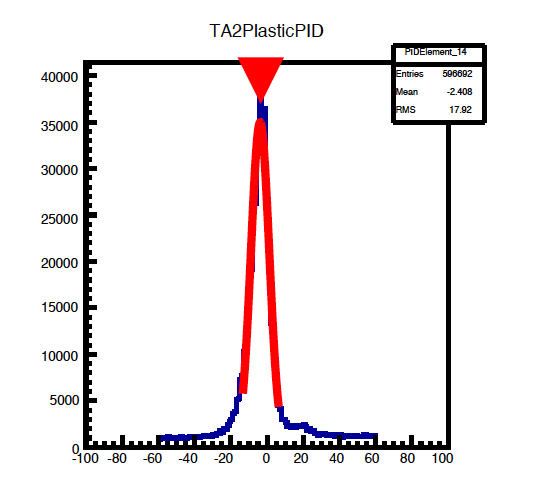
\includegraphics[scale=0.4]{pictures/png/pidtdcgaus.png}
\caption{Gaussian fit to PID-element 14.}
\label{pidtdcgaus}
\end{center}
\end{figure}

\begin{figure}[H]
\begin{center}
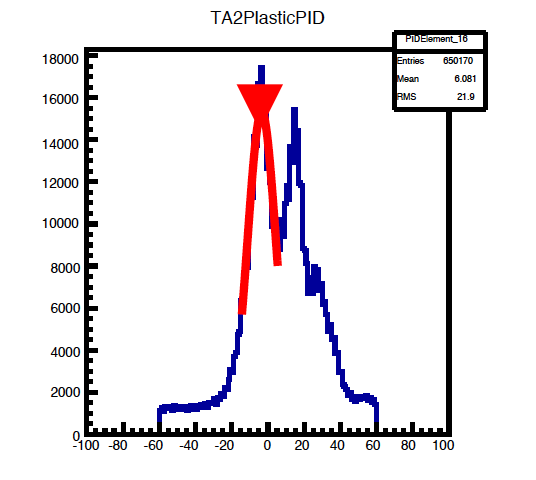
\includegraphics[scale=0.4]{pictures/png/pidtdcgaus16.png}
\caption{Gaussian fit to PID-element 16. The TDC spectrum of the malfunctioning PID element.}
\label{pidtdcgaus16}
\end{center}
\end{figure}

\begin{figure}[H]
\begin{center}
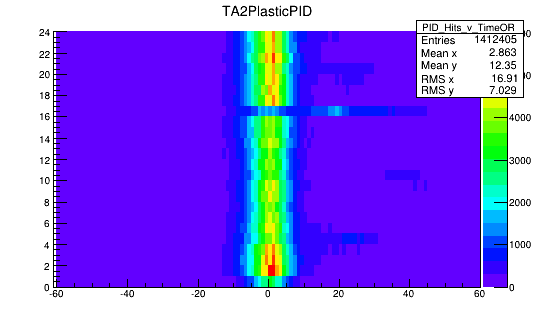
\includegraphics[scale=0.55]{pictures/png/pidtdcoffset.png}
\caption{Time alignment of all PID elements.}
\label{pidtdcoffset}
\end{center}
\end{figure}

\section{TAPS Calibration}

\indent The calibration of the TAPS BaF$_{2}$ crystals employed cosmic rays using the mean deposited energy of the minimum ionizing muons equal to 37.7MeV \cite{roebig}. For each of the BaF$_{2}$ crystals' PMTs the position of the energy peak has been adjusted so it was at the same ADC position for all detector elements, and the channel number corresponding to the mean peak position was determined.

\indent Using a similar technique to that employed in the CB calibrations, the correction for the gain was obtained. However, because detection of two photons from the $\pi^{0}$ in TAPS is very rare, the events having one photon detected in TAPS and one in CB were chosen. Detailed procedure of this calibration can be found in \cite{lemmer}.

\indent The procedure to calibrate plastic Veto was similar to the one used to calibrate PID. The pedestal positions were obtained from the raw ADC spectra and the gain was determined by comparing the experimental mean position of the proton peak in the Veto to the simulated data. Details of this method can be found in reference \cite{gessler}

\section{Target Position Correction}


   
%\section{section name}

%some shit

%\section{section name}
